\documentclass[aspectratio=169, 10pt]{beamer}
\usetheme{Madrid}
\usefonttheme{professionalfonts}

\usepackage[english]{babel}
\usepackage[linguistics]{forest}
\usepackage[utf8]{inputenc}
\usepackage{algorithmic}
\usepackage{amsfonts}
\usepackage{amsmath}
\usepackage{amssymb}
\usepackage{array}
\usepackage{bookmark}
% \usepackage{boondox-cal}
\usepackage{caption}
\usepackage{colortbl}
\usepackage{csquotes}
\usepackage{graphicx}
\usepackage{hyperref}
\usepackage{lipsum}
\usepackage{lmodern}
\usepackage{mathptmx}
\usepackage{mathtools}
\usepackage{multirow}
\usepackage{pgfplots}
\usepackage{svg}
\usepackage{xcolor}

% \pgfplotsset{compat=1.17}
\usetikzlibrary{calc}

\hypersetup{
    colorlinks=true,
    linkcolor=blue,
    filecolor=blue,      
    urlcolor=blue,
}

\title{Tutorial 4}
\subtitle{Supervised Learning using Neural Network}
\author{Luke Chang}
\institute{The University of Auckland}
\date{Mar. 2021}


\begin{document}

\frame{\titlepage}

%-------------------------------------------------------------------------------
\begin{frame}
    \frametitle{Objectives}

    \tableofcontents
        
\end{frame}

%-------------------------------------------------------------------------------
\section{Overview on Neural Network}
\begin{frame}
    \frametitle{Overview on Neural Network}

    Where does neural network (NN) shine?
    \begin{itemize}
        \item Commonly used in supervised learning where data has a lot of instances and feature space is large.
        \item It scales well when data size increases.
    \end{itemize}
    
    An (artificial) neural network is a direct graph.
    \begin{itemize}
        \item \textbf{Feed-forward neural network (FFNN):} A directed acyclic graph, where nodes are arranged in layers from inputs to outputs.
        \item \textbf{Recurrent neural network (RNN):} A directed graph with cycles; nodes have additionally feedback into themselves or previous nodes.
    \end{itemize}

    \begin{block}{Motivation}
        To combat \textbf{gradient vanishing} problem, \textit{feedback nodes} in the hidden layers are commonly used in large-scale deep neural networks.
    \end{block}
        
\end{frame}

%-------------------------------------------------------------------------------
\begin{frame}
    \frametitle{A basic NN with 1 hidden layer}
    
    \begin{itemize}
        \item The data has $n$ features, and the outputs have $m$ classes.
        \item $k$ hidden neurons in the hidden layer.
        \item Let $x$ be the input vector where $x \in \mathbb{R}^n$, hidden layer $h$ is a vector where $h \in \mathbb{R}^k$ and output $o$ is a vector where $o \in \mathbb{R}^m$.
        \item Nodes are connected by weights. These weights are learnt during the training. The weight matrices for the hidden layer is $W_0 \in \mathbb{R}^{k \times n}$, and for the output layer is $W_1 \in \mathbb{R}^{m \times k}$.
        \item Biases are $b_0 \in \mathbb{R}^k$ and $b_1 \in \mathbb{R}^m$, where $x_0 = h_0 = 1$.
    \end{itemize}

    \begin{figure}
        \centering
        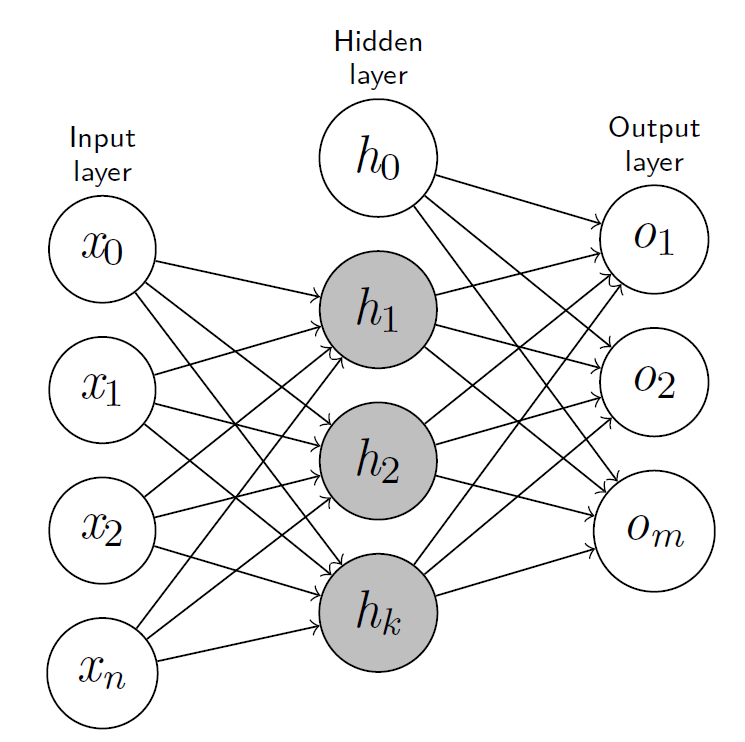
\includegraphics[width=0.18\columnwidth]{../imgs/nn_01.png}
    \end{figure}

    $o = f(W_1 \cdot f(W_0 \cdot x + b_0) + b_1)$, where $f$ is the activation function, applied element-wise.\\

    \textbf{Note:} The last activation function should based on the desired outputs. (Eg: One-hot encoding, regression)
        
\end{frame}

%-------------------------------------------------------------------------------
\section{Activation Functions}
\begin{frame}
    \frametitle{Activation Functions}
    
    The activation function must be \textbf{non-linear}.\break

    For a given non-input node $h$:
    \begin{itemize}
        \item Suppose there are $n$ nodes connect to $h$.
        \item Let $x$ be the column vector input to the node, that $x = (x_0, x_1, \ldots, x_n)^T$, where $x_0=1$.
        \item Let $w$ be the weights on the incident edges, that $w = (w_0, w_1, \ldots, w_n)^T$, where $w_0=b$ is the bias.
    \end{itemize}

    The output from this node is given by:

    \[
        f(w^T x) = f(\sum_{i=0}^n w_i x_i) = f(\sum_{i=1}^n w_i x_i + b)
    \]

    Where $f$ is the activation function for this node.\break

    If the activation function is linear, we can merge multiple hidden layers into one layer.
    The structure is equivalent to linear regression.
\end{frame}

%-------------------------------------------------------------------------------
\begin{frame}
    \frametitle{Sigmoid Function}

    \begin{figure}
        \centering
        \resizebox{0.35\columnwidth}{!}{
            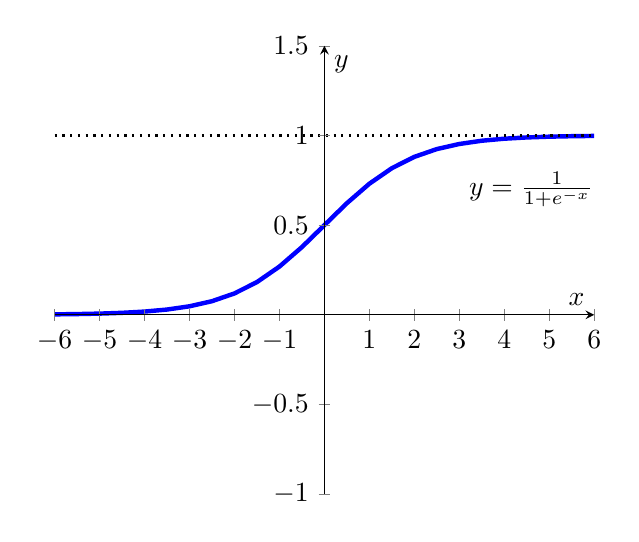
\begin{tikzpicture}
                \begin{axis}[
                        xmin=-6, xmax=6,
                        ymin=-1, ymax=1.5,
                        axis lines=center,
                        axis on top=true,
                        domain=-6:6,
                        ylabel=$y$,
                        xlabel=$x$,
                        xtick distance=1,
                        ytick distance=0.5
                    ]
                
                    \addplot [mark=none,draw=blue,ultra thick] {1/(1+exp(-\x))};
                    \node [right, black] at (axis cs: 3,0.7) {$y = \frac{1}{1+e^{-x}}$};
                    
                    \draw [black, dotted, thick] (axis cs:-6,1)-- (axis cs:6,1);
                    % \draw [black, dotted, thick] (axis cs:-6,0)-- (axis cs:6,0);
                \end{axis}
            \end{tikzpicture}    
        }
    \end{figure}

    \[
        f(x) = \text{Sigmoid}(x) = \sigma(x) = \frac{1}{1 + e^{-x}}
    \]

    Where $f(x) \in (0, 1)$, and the derivative is $f'(x) = f(x)(1- f(x))$.\\
    Rarely used in hidden layers for state-of-the-art models.\\
    Often used in the last hidden layer to produce logistic outputs.
\end{frame}

%-------------------------------------------------------------------------------
\begin{frame}
    \frametitle{Hyperbolic Tangent (tanh) Function}

    \begin{figure}
        \centering
        \resizebox{0.35\columnwidth}{!}{
            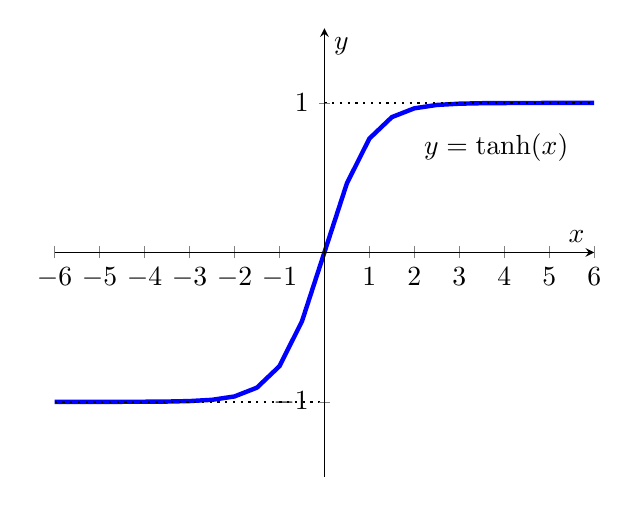
\begin{tikzpicture}
                \begin{axis}[
                        xmin=-6, xmax=6,
                        ymin=-1.5, ymax=1.5,
                        axis lines=center,
                        axis on top=true,
                        domain=-6:6,
                        ylabel=$y$,
                        xlabel=$x$,
                        xtick distance=1,
                        ytick distance=1
                    ]
                
                    \addplot [mark=none,draw=blue,ultra thick] {tanh(\x)};
                    \node [right, black] at (axis cs: 2,0.7) {$y = \tanh (x)$};
                    
                    \draw [black, dotted, thick] (axis cs:-6,-1)-- (axis cs:0,-1);
                    \draw [black, dotted, thick] (axis cs:0,1)-- (axis cs:6,1);
                \end{axis}
            \end{tikzpicture}    
        }
    \end{figure}

    \[
        f(x) = \tanh(x) = \frac{\sinh(x)}{\cosh(x)} = \frac{e^x - e^{-x}}{e^x + e^{-x}}
    \]
    
    Where $f(x) \in (-1, 1)$, and the derivative is $f'(x) = 1 - f(x)^2$\\
    Similar to Sigmoid function, but faster to converge.
\end{frame}

%-------------------------------------------------------------------------------
\begin{frame}
    \frametitle{Rectified Linear Unit (ReLU) Function}
    \small
    \begin{figure}
        \centering
        \resizebox{0.275\columnwidth}{!}{
            \begin{tikzpicture}
                \begin{axis}[
                        xmin=-2, xmax=2,
                        ymin=-1, ymax=2,
                        axis lines=center,
                        axis on top=true,
                        domain=-2:2,
                        ylabel=$y$,
                        xlabel=$x$,
                        xtick distance=1,
                        ytick distance=1
                    ]
                
                    \addplot+[mark=none,draw=blue,ultra thick,domain=-2:0] {0};
                    \addplot+[mark=none,draw=blue,ultra thick,domain=0:2] {\x};
                    
                \end{axis}
            \end{tikzpicture}    
        }
    \end{figure}

    \[
        f(x) = \text{ReLU}(x) = (x)^+ = \max(0, x)
    \]

    Where $f(x) \in [ 0, +\infty )$. The derivative is equal to:
    \[
        f'(x) = \begin{cases}
            0,& \text{if } x < 0 \\
            1,& \text{if } x > 0
        \end{cases}
    \]
    Where $x = 0$ is not differentiable.\\
    ReLU is the most common activation function for hidden layers in recent deep learning.

\end{frame}

%-------------------------------------------------------------------------------
\begin{frame}
    \frametitle{Leaky ReLU}
    \small
    \begin{figure}
        \centering
        \resizebox{0.275\columnwidth}{!}{
            \begin{tikzpicture}
                \begin{axis}[
                        xmin=-2, xmax=2,
                        ymin=-1, ymax=2,
                        axis lines=center,
                        axis on top=true,
                        domain=-2:2,
                        ylabel=$y$,
                        xlabel=$x$,
                        xtick distance=1,
                        ytick distance=1
                    ]

                    \node [right, black] at (axis cs: -2,-0.5) {$\epsilon = 0.1$};
                
                    \addplot+[mark=none,draw=blue,ultra thick,domain=-2:0] {0.1*\x};
                    \addplot+[mark=none,draw=blue,ultra thick,domain=0:2] {\x};
                    
                \end{axis}
            \end{tikzpicture}    
        }
    \end{figure}
    Let $\epsilon$ be the negative slope:
    \[
        f(x) = \text{LeakyReLU}(x) = \max(0, x) + \epsilon \times \min(0, x) = \begin{cases}
            x,& \text{if } x \geq 0\\
            \epsilon \times x,& \text{otherwise}
        \end{cases}
    \]
    Where $f(x) \in \mathbb{R}$, and $\epsilon \in [0, 1)$ The derivative is equal to ($x = 0$ is not differentiable):
    \[
        f'(x) = \begin{cases}
            \epsilon,& \text{if } x < 0 \\
            1,& \text{if } x > 0
        \end{cases}
    \]
    Similar to ReLU, but overcomes the ``dead neuron'' problem.
\end{frame}

%-------------------------------------------------------------------------------
\section{Loss Functions}
\begin{frame}
    \frametitle{Loss/Cost Functions - MSE}
    
    The goal of training is to minimize a loss function. 
    An objective function is a loss function.\break

    \textbf{Mean Squared Error (MSE)}
    \[
        l(X, y| W) = \text{MSE} = \frac{1}{N} \sum_{i=1}^{N}(y_i - \hat{y_i})^2
    \]

    \begin{itemize}
        \item Squared L2-norm error;
        \item Loss is computed forward,
        \item $W$ are the weights.
        \item $X$ are the data.
        \item $y$ are the target labels.
        \item Minimizing $l$ using backpropagation with stochastic gradient descent (SGD) algorithm.
    \end{itemize}
\end{frame}

%-------------------------------------------------------------------------------
\begin{frame}
    \frametitle{Mean Absolute Error (MAE)}
    
    \[
        l(X, y| W) = \text{MAE} = \frac{1}{N} \sum_{i=1}^{N}|y_i - \hat{y_i}|
    \]

    \begin{itemize}
        \item Minimizing L1-norm error
        \item Compare with MSE, L1-norm is more robust to outliers.
        \item Compare with MSE, the solution from L1-norm is unstable, so it is harder to optimize.
    \end{itemize}

    When use as regularization:
    \begin{itemize}
        \item L1-regularization prefers sparse outputs.
        \item L2-regularization prefers smaller weights and distributes the weights more evenly.
    \end{itemize}

\end{frame}

%-------------------------------------------------------------------------------
\begin{frame}
    \frametitle{Softmax Function}
    Softmax function is defined as:
    \[
        \text{Softmax}(x_i) = \frac{\exp(x_i)}{ \sum_j \exp(x_j)}
    \]

    \begin{itemize}
        \item The outputs from a NN can be negative or above 1.
        \item Softmax function rescales them so that the elements of a n-dimensional output lie in the range $[0, 1]$ and sum to 1.
    \end{itemize}
        
\end{frame}

%-------------------------------------------------------------------------------
\begin{frame}
    \frametitle{Negative Log Likelihood (NLL) Loss}

    NLL Loss is useful to train a classification problem with multiple output classes.\break

    Let $p$ be a vector of probabilities (after Softmax function). 
    \[
        p_k = \frac{\exp(f_k)}{\sum_j \exp(f_j)}
    \]

    The Loss for one example is:
    \[
        L_i = - \log(p_{y_i})
    \]

    The partial derivative is extremely simple:
    \[
        \frac{\partial L_i}{\partial f_k} = p_k - 1(y_i = k)
    \]

    Example:
    \begin{table}[]
        \begin{tabular}{ccc|c}
         & \textbf{Class} & \textbf{Prediction} & \textbf{df} \\ \hline
        Alpaca & 0 & 0.2 & \textbf{0.2} \\
        Cat & 1 & 0.3 & \textbf{-0.7} \\
        Dog & 0 & 0.5 & \textbf{0.5} \\       
        \end{tabular}
    \end{table}
        
\end{frame}

%-------------------------------------------------------------------------------
\section{Optimization}
\begin{frame}
    \frametitle{Optimization - Stochastic Gradient Descent (SGD)}
    \small
    
    \begin{itemize}
        \item Gradient Descent: Minimizing the loss function by computing the gradient of the error and adjust the weights to descend the landscape into an error minima.
        \item Iterative algorithm
        \item Starts from a random point and travels down its slope with \textbf{learning rate $\lambda$} until it reaches the lowest point.
        \item Stochastic Gradient Descent (SGD) - Stochastic means \textbf{random}; Randomly select one instance at each iteration to reduce the computation cost;
        \item SGD works well with \textbf{mini-batch}, where the entire training data is divided into multiple random batches (without replacement, usually between 32 and 256).
    \end{itemize}
    
    \begin{figure}
        \centering
        \resizebox{0.2\columnwidth}{!}{
            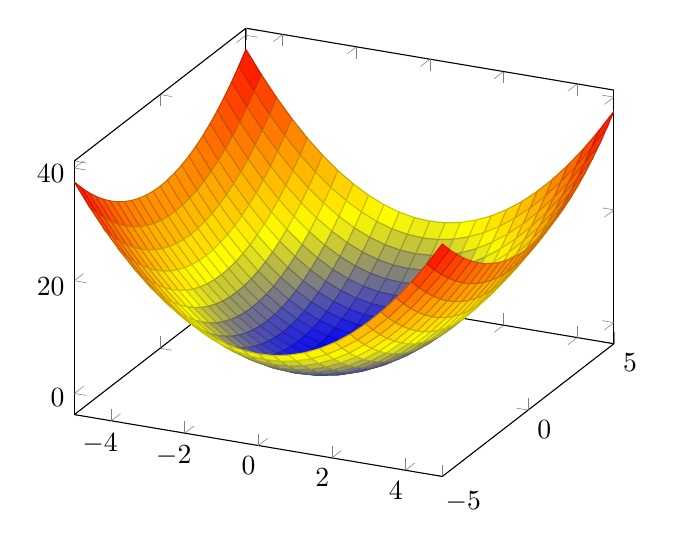
\begin{tikzpicture}
                \begin{axis}
                \addplot3[
                    surf,
                ]
                {x^2+0.5*y^2};
                \end{axis}
            \end{tikzpicture}
        }
    \end{figure}
    \begin{columns}
        \begin{column}{0.5\textwidth}
            \[
                \text{step\_size} = \text{gradient} \times \lambda
            \]
        \end{column}
        \begin{column}{0.5\textwidth}
            \[
                W^{[i+1]} = W^{[i]} - \text{step\_size}
            \]
        \end{column}
    \end{columns}

\end{frame}

%-------------------------------------------------------------------------------
\section{Different Types of Layers}
\begin{frame}
    \frametitle{Convolutional Neural Network (CNN) - Convolutional Layers}
    
    \begin{itemize}
        \item Convolutional Neural Network (CNN) is commonly applied to image datasets.
        \item CNN is a type of DNN.
        \item Convolutional layers is the fundamental building blocks for CNN.
        \item Convolutional layers convolve the input and pass its result to the next layer. (Convolution operation: $f*g$)
        \item Similar to apply an image filter, but all weights in the kernel are learnt during the training.
    \end{itemize}

    \begin{figure}
        \centering
        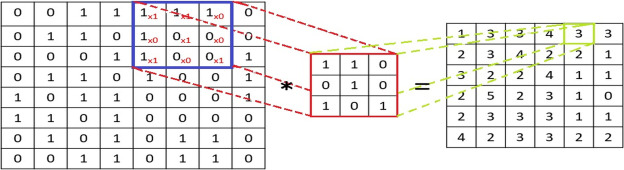
\includegraphics[width=0.3\columnwidth]{../imgs/conv.jpg}
    \end{figure}

    The height of the output is:
    \[
        H_{\text{out}} = \lfloor \frac{H_{\text{in}} - K + 2P}{S} + 1 \rfloor
    \]
    Where $K$ is kernel size, $S$ is stride, and $P$ is zero padding.\\
    The same formula is also applied to the output width.
\end{frame}

%-------------------------------------------------------------------------------
\begin{frame}
    \frametitle{Convolutional Neural Network (CNN) - Pooling Layers}
    \small
    Pooling layers of a CNN implement a spatial dimensionality reduction operation designed to reduce the number of trainable parameters for the next layers.\break

    Different types of pooling layer:
    \begin{itemize}
        \item Average pooling
        \item Max. pooling
        \item Adaptive max. pooling: Similar to Max. pooling, but define \texttt{output\_size} instead of kernel size.
    \end{itemize}

    \begin{figure}
        \centering
        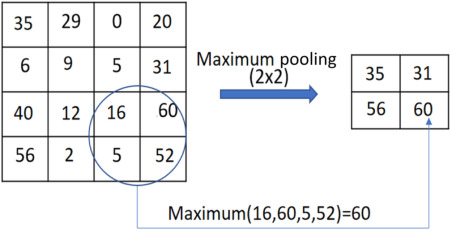
\includegraphics[width=0.27\columnwidth]{../imgs/max_pool.jpg}
    \end{figure}

    \begin{figure}
        \centering
        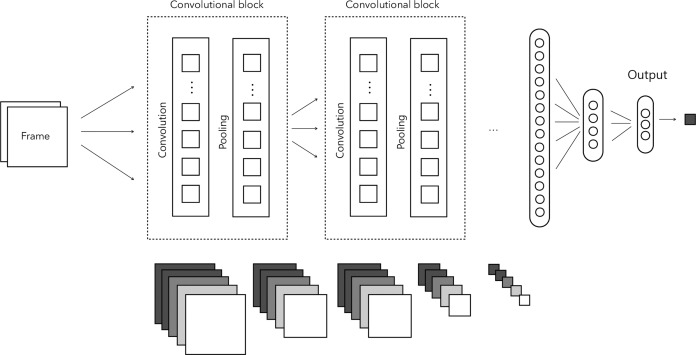
\includegraphics[width=0.37\columnwidth]{../imgs/image_nn.jpg}
    \end{figure}
\end{frame}

%-------------------------------------------------------------------------------
\section{Tutorial Questions}
\begin{frame}
    \frametitle{Tutorial Questions for Neural Networks}

    \begin{block}{Question 1}
        Suppose you have a fully connected Neural Network with 2 variable inputs, 1 hidden layer with 3 nodes and an output layer with 4 nodes.
    \end{block}

    \begin{itemize}
        \item How many weights will you learn? \onslide<2->{{\color{red}$2 \times 3 + 3 \times 4 = 18$}}
        \item What will be the hypothesis returned by this neural network? \onslide<3->{{\color{red}$3 + 4 = 7$ biases; $7+18=25$; A matrix of 25 numbers}}
        \item What will be the hypothesis space? \onslide<4->{{\color{red}25-dimensional space of real numbers}}
        \item If you add a second hidden layer to the neural network above, also with 3 nodes, how many weights will we learn? \onslide<5->{{\color{red}$2\times 3 + 3\times 3 + 3\times 4 = 27$}}
        \item Which NN will be more apt to over fit? \onslide<6->{{\color{red}The 2nd one, because it has more degrees of freedom.}}
    \end{itemize}
\end{frame}

%-------------------------------------------------------------------------------
\begin{frame}
    \frametitle{Tutorial Questions for Genetic Algorithms}

    \begin{block}{Question 1}
        Suppose you have a population of two individuals 111111 and 101010.    
    \end{block}

    How many applications of:
    \begin{itemize}
        \item single-point mutation would it take to get to 101111? \onslide<2->{{\color{red} 1}}
        \item single-point crossover would it take to get to  101111? \onslide<3->{{\color{red} 1}}
        \item two-point crossover would it take to get to  101111? \onslide<4->{{\color{red} 1}}
        \item single-point mutation would it take to get to  111011? \onslide<5->{{\color{red} 1}}
        \item single-point crossover would it take to get to  111011? \onslide<6->{{\color{red} 2}}
        \item two-point crossover would it take to get to  111011? \onslide<7->{{\color{red} 1}}
        \item single-point mutation would it take to get to  010101? \onslide<8->{{\color{red} 3}}
        \item single-point crossover would it take to get to  010101? \onslide<9->{{\color{red} Infinite}}
        \item two-point crossover would it take to get to  010101? \onslide<10->{{\color{red} Infinite}}
    \end{itemize}
\end{frame}

%-------------------------------------------------------------------------------
\begin{frame}
    \frametitle{Tutorial Questions for Genetic Algorithms}

    \begin{block}{Question 2}
        A population of two individuals 111111 and 101010. 
        And the probability of choosing each parent is $1/2$ and the probability of choosing mutation, 
        single-point crossover or two-point crossover is $1/3$. 
        The mutation flips the bit and has a uniform chance of being applied to each bit. 
        Single-point and two-point crossover have a uniform chance of choosing each location. 
        Once crossover or mutation is done there is a 50\% of replacing each parent randomly.
    \end{block}

    \begin{itemize}
        \item What is the probability of getting 101111 by an application of mutation?
        \onslide<2->{{\color{red} $\frac{1}{2} \times \frac{1}{3} \times \frac{1}{6} \approx 0.0278 = 2.78\%$}}
        \item What is the probability of getting 101111 by an application of single-point crossover?
        \onslide<3->{{\color{red} $ 2 \times (\frac{1}{2} \times \frac{1}{2} \times \frac{1}{3} \times \frac{1}{6}) \approx 0.0278 = 2.78\%$}}
        \item What is the probability of getting 101111 by an application of two-point crossover?
        \onslide<4->{{\color{red} $\frac{1}{2} \times \frac{1}{2} \times \frac{1}{3} \times \frac{1}{6} \times \frac{2}{6} \approx 0.46296\%$}}
        \item What is the combined probability?
        \onslide<5->{{\color{red} $2.77 + 1.38 + 0.46296 \approx 4.61\%$}}
    \end{itemize}
    
\end{frame}

%-------------------------------------------------------------------------------
\begin{frame}
    \frametitle{Tutorial Questions for Genetic Algorithms}

    \begin{block}{Question 3}
        A population of two individuals 111111 and 101010. 
        And the probability of choosing each parent is $1/2$ and the probability of choosing mutation, 
        single-point crossover or two-point crossover is $1/3$. 
        The mutation flips the bit and has a uniform chance of being applied to each bit. 
        Single-point and two-point crossover have a uniform chance of choosing each location. 
        Once crossover or mutation is done there is a 50\% of replacing each parent randomly.
    \end{block}

    \begin{itemize}
        \item What is the probability of getting 111011 by an application of mutation?
        \onslide<2->{{\color{red} $\frac{1}{2} \times \frac{1}{3} \times \frac{1}{6} \approx 2.78\%$}}
        \item What is the probability of getting 111011 by an application of single-point crossover?
        \onslide<3->{{\color{red} $2 \times (\frac{1}{2} \times \frac{1}{2} \times \frac{1}{3} \times \frac{1}{6} \times \frac{1}{2} \times \frac{1}{2} 
            \times \frac{1}{2} \times \frac{1}{3} \times \frac{1}{6}) \approx 0.01929\%$}}
        \item What is the probability of getting 111011 by an application of two-point crossover?
        \onslide<4->{{\color{red} $\frac{1}{2} \times \frac{1}{2} \times \frac{1}{3} \times \frac{1}{6} \times \frac{1}{6} \approx 0.23148\%$}}
    \end{itemize}
    
\end{frame}

%-------------------------------------------------------------------------------
\begin{frame}
    \frametitle{Tutorial Questions for Genetic Algorithms}

    \begin{block}{Question 4}
        A population of two individuals 111111 and 101010. 
        And the probability of choosing each parent is $1/2$ and the probability of choosing mutation, 
        single-point crossover or two-point crossover is $1/3$. 
        The mutation flips the bit and has a uniform chance of being applied to each bit. 
        Single-point and two-point crossover have a uniform chance of choosing each location. 
        Once crossover or mutation is done there is a 50\% of replacing each parent randomly.
    \end{block}

    \begin{itemize}
        \item What is the probability of getting 010101 by an application of mutation?
        \onslide<2->{{\color{red} $
            \frac{1}{2} \times \frac{1}{3} \times \frac{1}{6} \times \frac{1}{6} \times \frac{1}{2} \times \frac{1}{2} \times \frac{1}{3} \times \frac{1}{6} \times
            \frac{1}{6} \times \frac{1}{2} \times \frac{1}{2} \times \frac{1}{2} \times \frac{1}{3} \times \frac{1}{6} \times \frac{1}{6} \times \frac{1}{2}
            \approx 0.0000006201814\%
        $}}
        \item What is the probability of getting 010101 by an application of single-point crossover?
        \onslide<3->{{\color{red} Requires infinite applications, so 0\%}}
        \item What is the probability of getting 010101 by an application of two-point crossover?
        \onslide<3->{{\color{red} Requires infinite applications, so 0\%}}
    \end{itemize}
    
\end{frame}

\end{document}
